% ==============================================================================
% Chandigarh University Professional Resume Template
% Format: Two-column ATS-friendly layout
% ==============================================================================

\documentclass[10pt,a4paper]{article}

\usepackage[T1]{fontenc}
\usepackage[utf8]{inputenc}

\usepackage[
    left=0.45cm,
    right=0.45cm,
    top=0.35cm,
    bottom=0.35cm
]{geometry}

\usepackage[T1]{fontenc}
\usepackage{lmodern}
\usepackage{anyfontsize}
\usepackage{graphicx}
\usepackage{xcolor}
\usepackage{enumitem}
\usepackage[hidelinks]{hyperref}
\usepackage{titlesec}
\usepackage{paracol}

\pagestyle{empty}
\setlength{\parindent}{0pt}
\renewcommand{\familydefault}{\sfdefault}

% ================= COLOR DEFINITIONS =================
\definecolor{mainred}{HTML}{800000} % CU Dark Maroon
\definecolor{dividerorange}{HTML}{D2691E}

% ================= SECTION FORMATTING =================
\titleformat{\section}
{\color{mainred}\bfseries\fontsize{10.5}{12}\selectfont\uppercase}
{}{0pt}{}
[\vspace{-2pt}\titlerule]

\titlespacing{\section}{0pt}{8pt}{4pt}

% ================= BULLET SETTINGS =================
\setlist[itemize]{
    leftmargin=0.65cm,
    itemsep=1.5pt,
    parsep=0pt,
    topsep=2pt,
    partopsep=0pt
}

% ================= PARACOL SETUP =================
\columnratio{0.32}
\setlength{\columnsep}{0.04\textwidth}
\setlength{\columnseprule}{1.2pt}
\colseprulecolor{dividerorange}

\begin{document}

\fontsize{9.2}{11}\selectfont

\begin{paracol}{2}

% ==============================================================================
%                                LEFT COLUMN
% ==============================================================================
\vspace*{0pt}

% --- PROFILE PICTURE INSTRUCTIONS ---
% 1. Upload your passport-size image to the same folder as this .tex file.
%
% 2. Replace 'profile-placeholder.jpg' below with your actual image filename.
%
% 3. The image automatically fits inside a 3.2cm × 3.2cm box without stretching
%    because 'keepaspectratio' preserves the original image proportions.
%
% 4. A thin professional border is added around the image to improve visibility
%    on white resume backgrounds and give a passport-photo appearance.
%
% 5. If your uploaded image already contains a border/frame, remove or comment
%    out the \fbox{...} wrapper below to avoid getting a double border effect.
%
% 6. Supported image formats: .jpg, .jpeg, .png

\setlength{\fboxsep}{0.5pt}      % Space between image and border
\setlength{\fboxrule}{0.2pt}   % Border thickness

\begin{center}

    \fbox{
        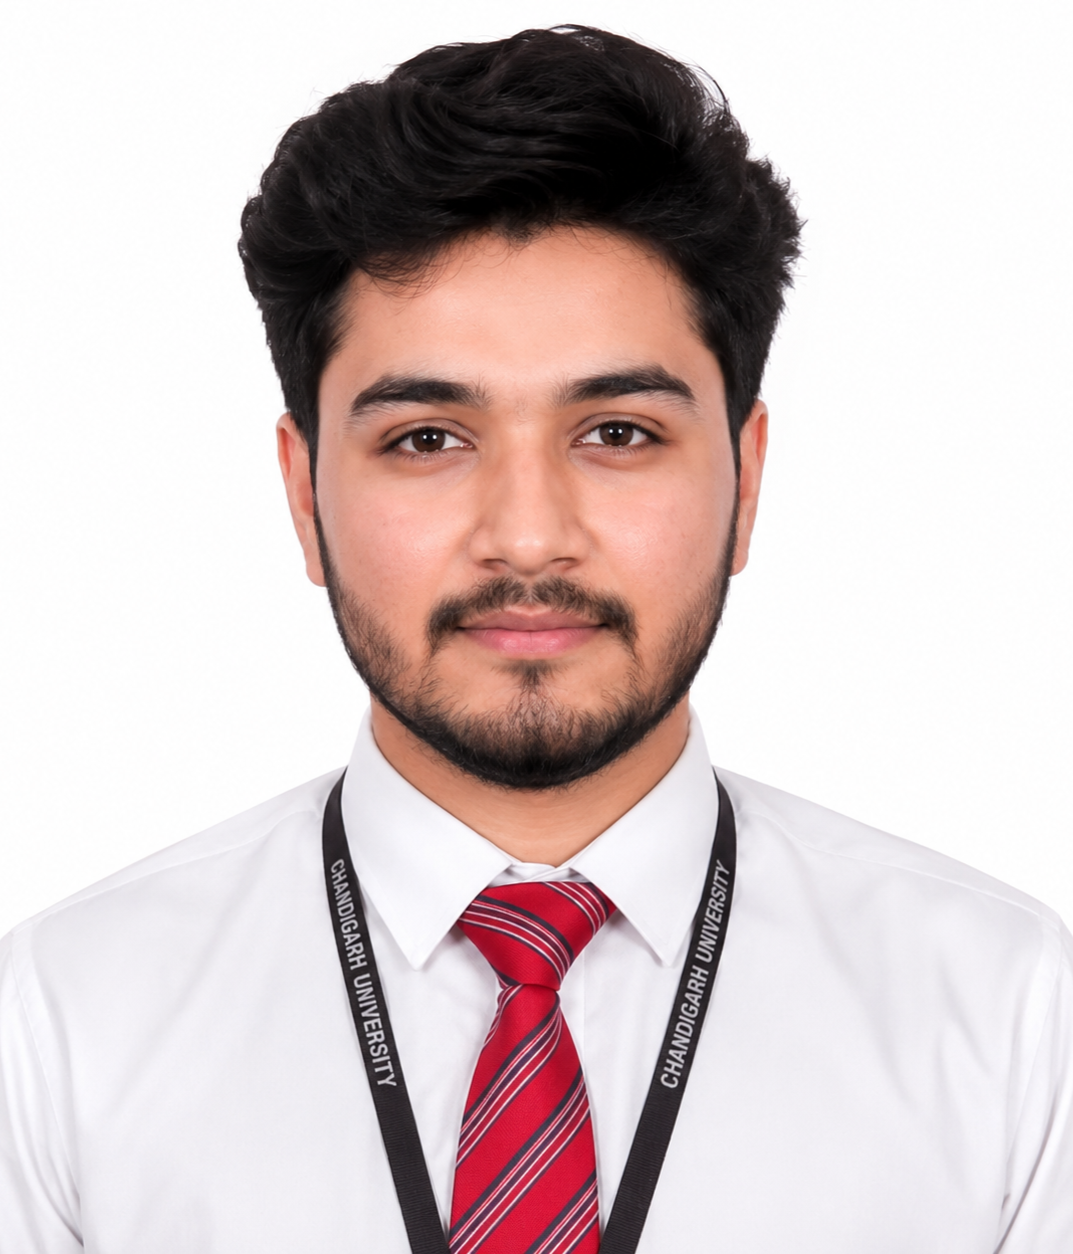
\includegraphics[
            width=3.2cm,
            height=3.2cm,
            keepaspectratio
        ]{profile-placeholder.jpg}
    }

\end{center}

\vspace{0.1cm}

\begin{center}
{\fontsize{18}{20}\selectfont \bfseries \color{mainred} RAHUL VERMA}
\end{center}

{\color{mainred}\rule{\linewidth}{0.8pt}}

\vspace{0.1cm}

\raggedright
\color{black}

\textbf{Address:} Sector 15, Chandigarh, (160015) \\[3pt]
\textbf{E-mail:} rahul.verma.21bcs@cuchd.in \\[3pt]
\textbf{Phone:} +91 98765 43210 \\[3pt]
\textbf{LinkedIn:} \href{https://linkedin.com/in/rahulverma}{in/@RahulV2025}

\section*{Professional Summary}
Results-driven Computer Science Engineering undergraduate specializing in full-stack web development and scalable backend systems. Proven ability to optimize database performance, integrate secure REST APIs, and build impactful browser extensions. Seeking a software engineering role to deliver user-centric solutions within a collaborative, fast-paced environment.

\section*{Technical Competencies}
\textbf{Languages:} Java, Python, C++, JavaScript (ES6+), TypeScript\\[4pt]
\textbf{Frameworks:} React.js, Node.js, Express.js, Next.js\\[4pt]
\textbf{Database:} MySQL, MongoDB, PostgreSQL, Firebase\\[4pt]
\textbf{Developer Tools:} Git, Docker, VS Code, Postman, AWS\\[4pt]
\textbf{Core Concepts:} Data Structures \& Algorithms, DBMS, OOP, Operating Systems

\section*{Interpersonal Skills}
Problem Solving \textbar{} Analytical Thinking \textbar{} Cross-functional Collaboration \textbar{} Agile Adaptability \textbar{} Time Management

\section*{Interests \& Hobbies}
Open Source Contribution \textbar{} Tech Community Mentorship \textbar{} Photography \textbar{} Chess

\section*{Languages Known}
English (Fluent) \textbar{} Hindi (Native) \textbar{} Punjabi (Conversational)

\switchcolumn

% ==============================================================================
%                                RIGHT COLUMN
% ==============================================================================
\vspace*{0pt}
\raggedright

\section*{Education}
\textbf{B.Tech in Computer Science Engineering} \textbar{} \textbf{Chandigarh University}, Punjab \\
\textit{Session: 2021-2025 \textbar{} CGPA: 8.65/10}

\vspace{5pt}
\textbf{Intermediate (CBSE)} \textbar{} Government Model Senior Secondary School, Chandigarh \\
\textit{Session: 2020-2021 \textbar{} Percentage: 89.40\%}

\vspace{5pt}
\textbf{Matriculation (CBSE)} \textbar{} St. Stephen's School, Chandigarh \\
\textit{Session: 2018-2019 \textbar{} Percentage: 93.20\%}

\section*{Experience \& Training}
\textbf{Software Development Intern \textbar{} Netsmartz Infotech Pvt. Ltd.} \hfill \textit{May 2024 -- Jul 2024}
\begin{itemize}
\item Developed RESTful APIs using Node.js and Express.js for internal enterprise management systems.
\item Optimized MongoDB indexing, reducing backend database query response times by 25\%.
\item Collaborated with UI/UX and frontend teams to integrate robust authentication middleware.
\item Participated in daily Agile stand-ups and managed version control workflows using Git/GitHub.
\end{itemize}

\section*{Projects}

\textbf{Developer Productivity Extension \textbar{} JavaScript \& Chrome APIs} \hfill \textit{Jan 2024 -- Mar 2024}
\begin{itemize}
\item Engineered a lightweight browser extension automating repetitive code-formatting tasks across web IDEs.
\item Achieved high community impact, successfully scaling the tool to over 1,000 active daily users.
\item Implemented local storage caching to maintain user preferences and ensure zero-latency loading.
\end{itemize}

\vspace{4pt}
\textbf{Smart Campus Management System \textbar{} MERN Stack} \hfill \textit{Sep 2023 -- Dec 2023}
\begin{itemize}
\item Built a comprehensive role-based platform for handling university attendance, notices, and academics.
\item Secured REST API endpoints using JWT authentication and bcrypt password hashing.
\item Designed a responsive, Google-style minimalist user interface using React and Tailwind CSS.
\end{itemize}

\vspace{4pt}
\textbf{Malicious URL Detection Engine \textbar{} Python \& ML} \hfill \textit{Apr 2023 -- Jul 2023}
\begin{itemize}
\item Trained a Random Forest classification model using Scikit-learn to detect phishing and malicious links.
\item Processed and extracted features from datasets containing over 50,000 URL samples.
\item Attained a 93.4\% prediction accuracy rate, deploying the final model via a lightweight Flask API.
\end{itemize}

\vspace{4pt}
\textbf{E-Commerce Web Application \textbar{} Next.js \& Firebase} \hfill \textit{Dec 2022 -- Feb 2023}
\begin{itemize}
\item Developed a responsive e-commerce platform featuring secure authentication and product management.
\item Integrated Firebase Authentication and Cloud Firestore for real-time database syncing.
\item Improved SEO performance and optimized client-side page rendering speeds using Next.js.
\end{itemize}

\section*{Academic Achievements}
\begin{itemize}
\item Recognized as a student contributor for \textbf{Google Summer of Code (GSoC) 2023}.
\item Qualified for Round 2 in the \textbf{Meta Hacker Cup 2023} global competitive programming contest.
\item Solved 500+ algorithmic and data structure challenges across LeetCode, HackerRank, and GeeksforGeeks.
\item Consistently ranked among the top 5\% of the batch in departmental competitive coding assessments.
\end{itemize}

\section*{Certifications}

\begin{itemize}
    \item \textbf{AWS Certified Solutions Architect – Associate} \hfill Amazon Web Services (AWS) | 2025
    \item \textbf{Microsoft Certified: Azure Fundamentals (AZ-900)} \hfill Microsoft | 2025
    \item \textbf{Oracle Certified Professional: Java SE Developer} \hfill Oracle | 2024
    \item \textbf{Google Associate Cloud Engineer} \hfill Google Cloud | 2025
\end{itemize}

\section*{Publications}

\begin{itemize}
    \item \textbf{SS-HCNN: Semi-Supervised Hierarchical Convolutional Neural Network for Image Classification} \\
    IEEE Transactions on Image Processing (IEEE TIP), 2018 \\
    DOI: 10.1109/TIP.2018.2886758 \\
    Link: \url{https://doi.org/10.1109/TIP.2018.2886758}
\end{itemize}

\end{paracol}
\end{document}